\setcounter{section}{3}
\setcounter{subsection}{1}

\subsection{Interprocess Dependencies}
This section will cover the design of the dynamic behaviour of the system through description, sequence diagrams and activity diagrams. It will start by looking at the android application.

\begin{figure}[h!]
    \centering
    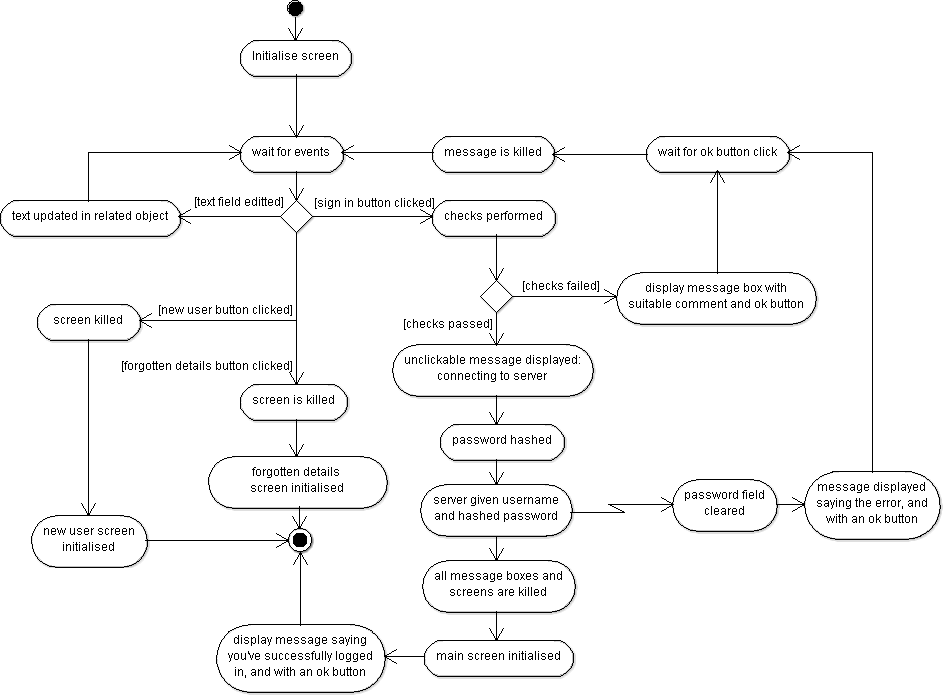
\includegraphics[width=0.9\textwidth]{images/activity/main-login}
    \caption{Activity diagram for the main login screen.}
    \label{fig:mainLogin}
\end{figure}

When a user first starts the app they will be taken to the main login screen. Figure \ref{fig:mainLogin} shows what can happen from this screen. Firstly the screen is initialised and graphics, buttons and text fields are put in the grid that makes up the view. After this the app will wait for events from the user, these include typing into the text fields and clicking buttons. If text is typed it is saved in the relevant text field and if the new user button or forgotten details button are clicked then the main login screen is killed and the relevant screen is initialised. However if the sign in button is clicked, the following processes are a bit more complex. Firstly the text fields are checked and if they are null a message is displayed. This message box will have an OK button that once clicked will kill the message box and the app will wait for more events. If the text fields aren't empty then the password is hashed and the hash and username is given to the server. If there are any errors connecting to the server or creating the user session then a message box with be displayed with the error and an OK button. If not the user will be logged on and shown the main screen and a message box saying successfully logged on, with an OK button. This satisfies requirement 5.1.5 user authentication.

Similar processes will occur for creating a new account from the new user screen, except the checks performed include making sure text fields aren't null, the username and password are 5-16 characters long, the password and check password fields contain the same String as the email and confirm email fields, the password has a letter and digit and the email is valid. In this case the server will be given the username and email as well as the hashed password and if there are no errors with the server the user will be shown the main login screen with a message telling them that an email has been sent to them to activate their new account. This satisfies requirement 5.1.1 account registration.

There are also few differences when a user has forgotten their password and has clicked the forgotten password button. The email address text field must be checked to see if a valid email has been entered. If the server request is successful then the user will be shown the main login screen with a message telling them that an email has been sent to them with a link to refresh their password. This satisfies requirement 5.1.8 password reset.

\begin{figure}[h!]
    \centering
    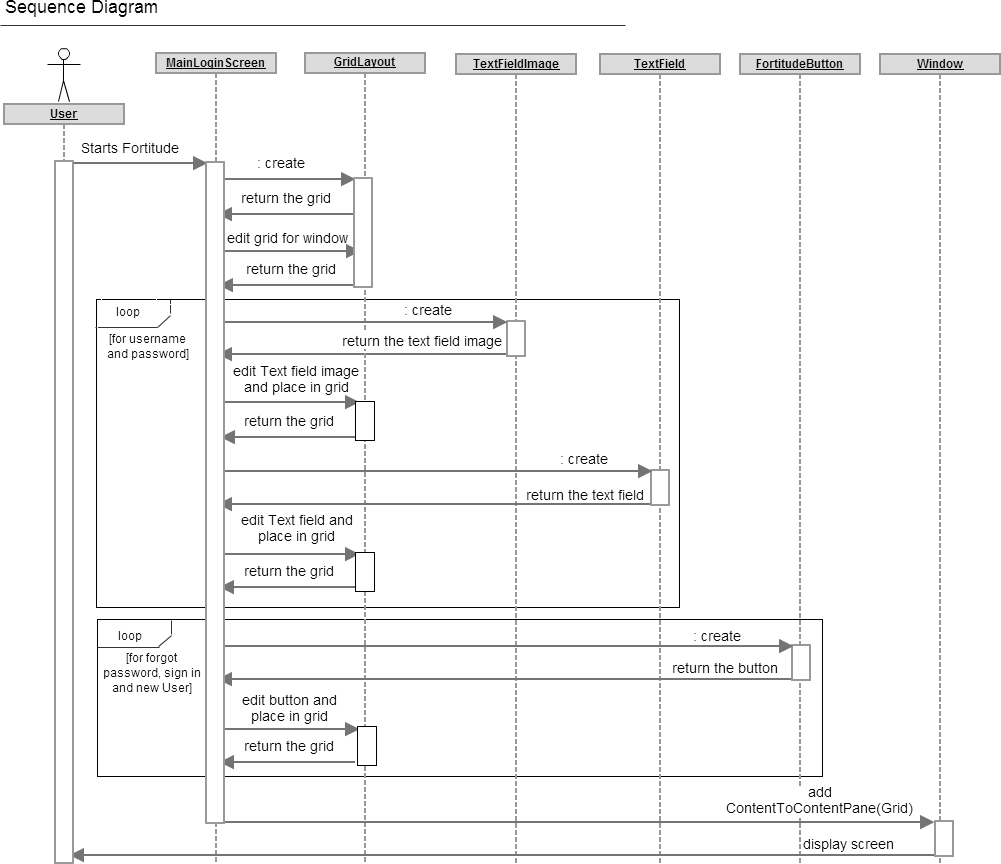
\includegraphics[width=0.9\textwidth]{images/sequence/createMainLoginScreen}
    \caption{Sequence diagram for the construction of the main login screen.}
    \label{fig:createLogin}
\end{figure}

Figure \ref{fig:createLogin} shows what happens in each of the classes when the main login screen is initialised. It is very similar for all screens. Once a new MainLoginScreen is created, the grid which everything sits on is initialised in the GridLayout class. The MainLoginScreen transforms the grid so it has enough squares and is the right size. Instances of TextFieldImage and TextField are initialised, edited and placed in the grid for username and password. Then the buttons for forgot password, sign in and new User are initialized in FortitudeButton, edited in the MainLoginScreen and placed in the grid. This grid is put in the window using a method in the Window class and this method displays the window to the user. When creating the grid and everything that goes in it the sizes are decided on the window size so nothing will be off the screen, satisfying requirement 5.3.8.

Figure \ref{fig:signIn} shows the sequence of events when the sign in button on the main login screen is pressed. Firstly the MainLoginScreen will call the method signIn(). It checks to see if the text fields aren't empty and displays a message box if they are. If not a message box saying connecting to server will appear which should satisfy requirement 5.3.9 as the rest may take a while to be performed but the user will see the message box nearly instantly. Next initialLogin() is called in the Login class which will hash the password and give the username and hashed password to ServerRequests. This will create an object of type RequestThread and call setURL() to give it a URL with all relevant information. This object connects to the server using the JSON parsing module and will analyse the response. JSON is used because it is very `light weight' to satisfy requirement 5.2.30. In the diagram I've just talked about a successful response. However if an error occurs the response will show this so ServerRequests can create a MessageBox with different text and not create a CurrentUser or display the main screen. But if the response is a success then these things will happen and a message with an OK button will be displayed that tells the user they've successfully logged on. This class diagram is very similar to other processes in the app as values are always checked in the current screen and the ServerRequests and RequestThread class as well as the JSON parsing module are used for most actions with a different method call in ServerRequests, therefore I will not include further class diagrams exactly how methods in ServerRequests work. Values are also checked by the server, however they are initially checked by the application as it will not take much processing time so the user will get a faster response if they've made a mistake.

\begin{landscape}
\begin{figure}
    \centering
    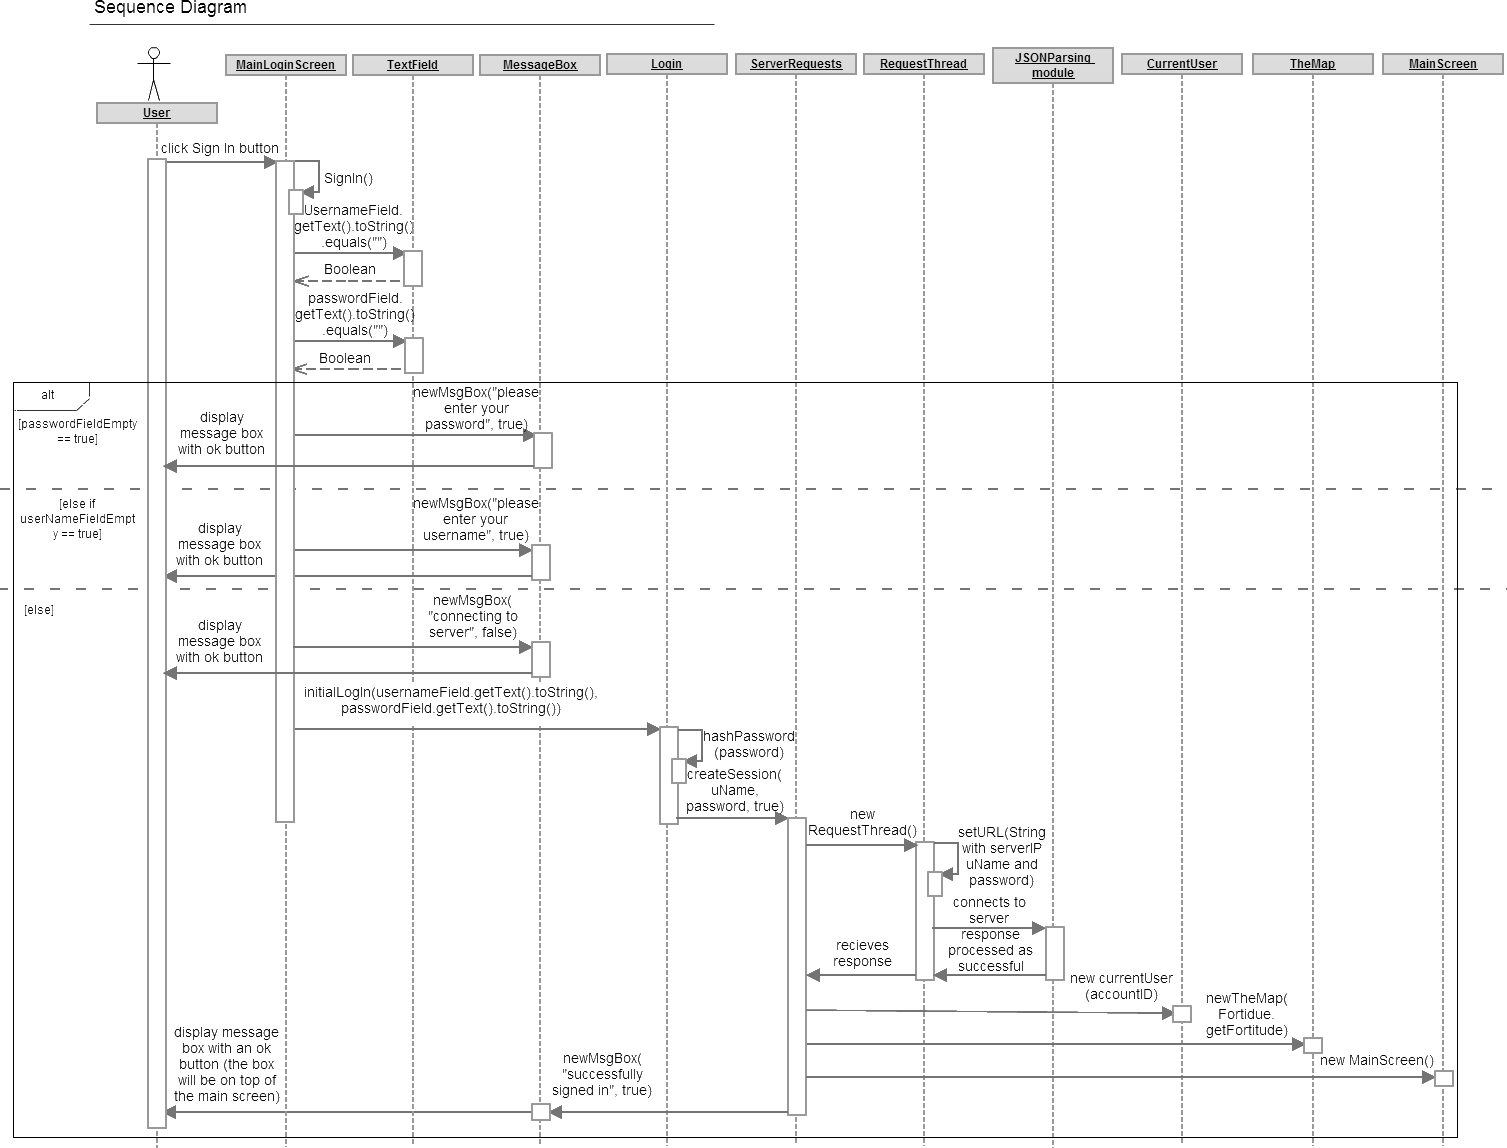
\includegraphics[height=0.9\textwidth]{images/sequence/signInbutton}
    \caption{Sequence diagram for the sign in button.}
    \label{fig:signIn}
\end{figure}
\end{landscape}

\begin{wrapfigure}{r}{0.56\textwidth}
    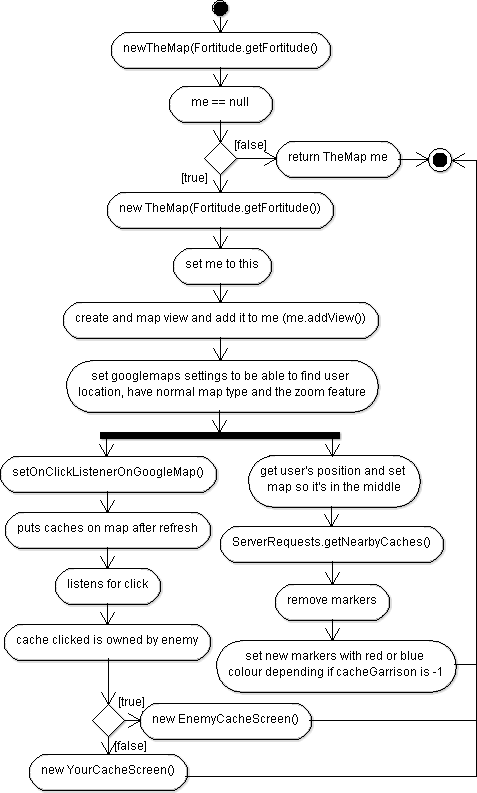
\includegraphics[width=0.56\textwidth]{images/activity/newMap}
    \caption{Activity diagram for construction of the map view.}
\end{wrapfigure}

Before the main screen is shown the map must be created as it is viewed on the main screen. If it has already been created it is returned else a new map is created. When this happens a map view is created and added to the map and particular Google map settings are enabled, including zooming to satisfy requirement 5.3.3. Then threading is used to run two parallel processes, one gets the users position and set's the map to be showing this position, (satisfying requirement 5.3.1) get's nearby caches and set's them as markers on the map with different colours and types relating to owners and cache types, to satisfy requirement 5.2.26. This has a separate method so that caches can be loaded around the user's position when requested to satisfy requirement 5.3.2. When getting the nearby non-player caches, it will only put them on the map if the user hasn't attacked it for a certain amount of time, satisfying requirement 5.2.19. The other parallel process deals with user interactions, putting caches on the map after the user refreshes it and listens for when the user clicks a cache to bring up a new related screen.

If a user has logged on before they will be automatically signed into that account again as shown in figure \ref{fig:autosave}. After the MainLoginScreen has been initialised it will create an instance of FileSave and use it to get username and password hash in String form the byte form in files that the app stores. If the username and password aren't null or empty then the ServerRequests class can create a session for the user from them, and take the user to the main screen. However if the username and password are empty or null then nothing will happen and the user will not be told they are connecting to the server but shown the main login screen. When a user logs out through the AccountScreen, their username and password are put as the empty string using the createDialog() method in FileSave.

If a user's account is not already activated then the bottom bar in the main screen will not have the normal buttons but instead have a button to take the user to the ActivateUserScreen. From this screen the user can click a button to resend the activation email which uses resendActivationEmail() in ServerRequests with the email of the account. This satisfies requirement 5.1.4.

\begin{wrapfigure}{l}{0.63\textwidth}
    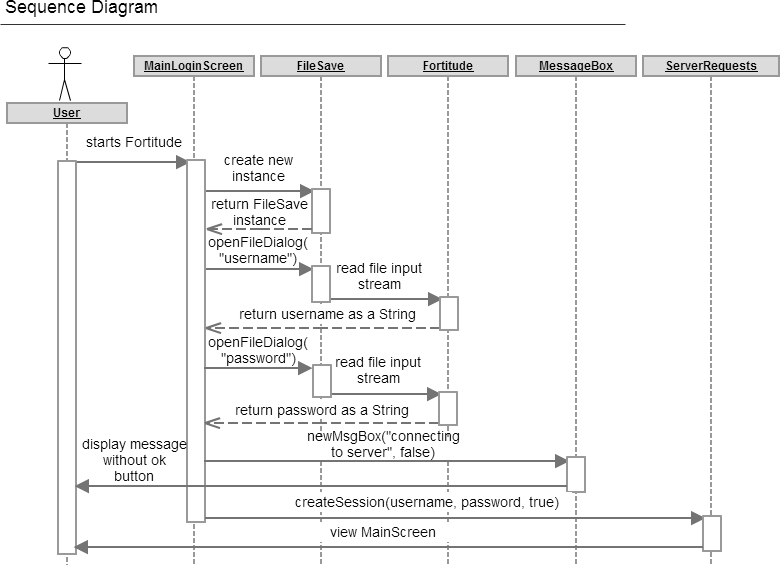
\includegraphics[width=0.63\textwidth]{images/sequence/autosave}
    \caption{Sequence diagram for the credential autosave feature.}
    \label{fig:autosave}
\end{wrapfigure}

\noindent
The sequence diagram for clicking the castle button is more complicated than for clicking other buttons so is shown in figure \ref{fig:castleButton}. For these events to occur the castle button must be clickable. If the castle is clickable a message is shown telling the user they're being connected to the server. Then refreshData() is called in the ServerRequests class to make sure all information including cache positions and user data is up to date. refreshData() can update a route to a cache too if there is one. If this request isn't successful then a message with an OK button is displayed to the user that says loading caches failed. If the request is successful then the latitudes and longitudes are found out for the user's current position and caches on the map and nearest cache and distance to it is calculated. If the closest cache isn't close enough then user is shown a message box with an OK button that tells them to get closer to the cache. Otherwise if the cache is owned by them they go to the visit your cache screen, which will show the cache balance satisfying requirement 5.2.4. However, if the cache isn't owned by them they go to the visit enemy cache screen which will say the owner of the cache. If it's a non-player cache the visit enemy cache screen is still used, however it will not have the owner of the cache on. This will satisfy requirement 5.2.3, cache ownership.

\newpage
\begin{figure}
    \centering
    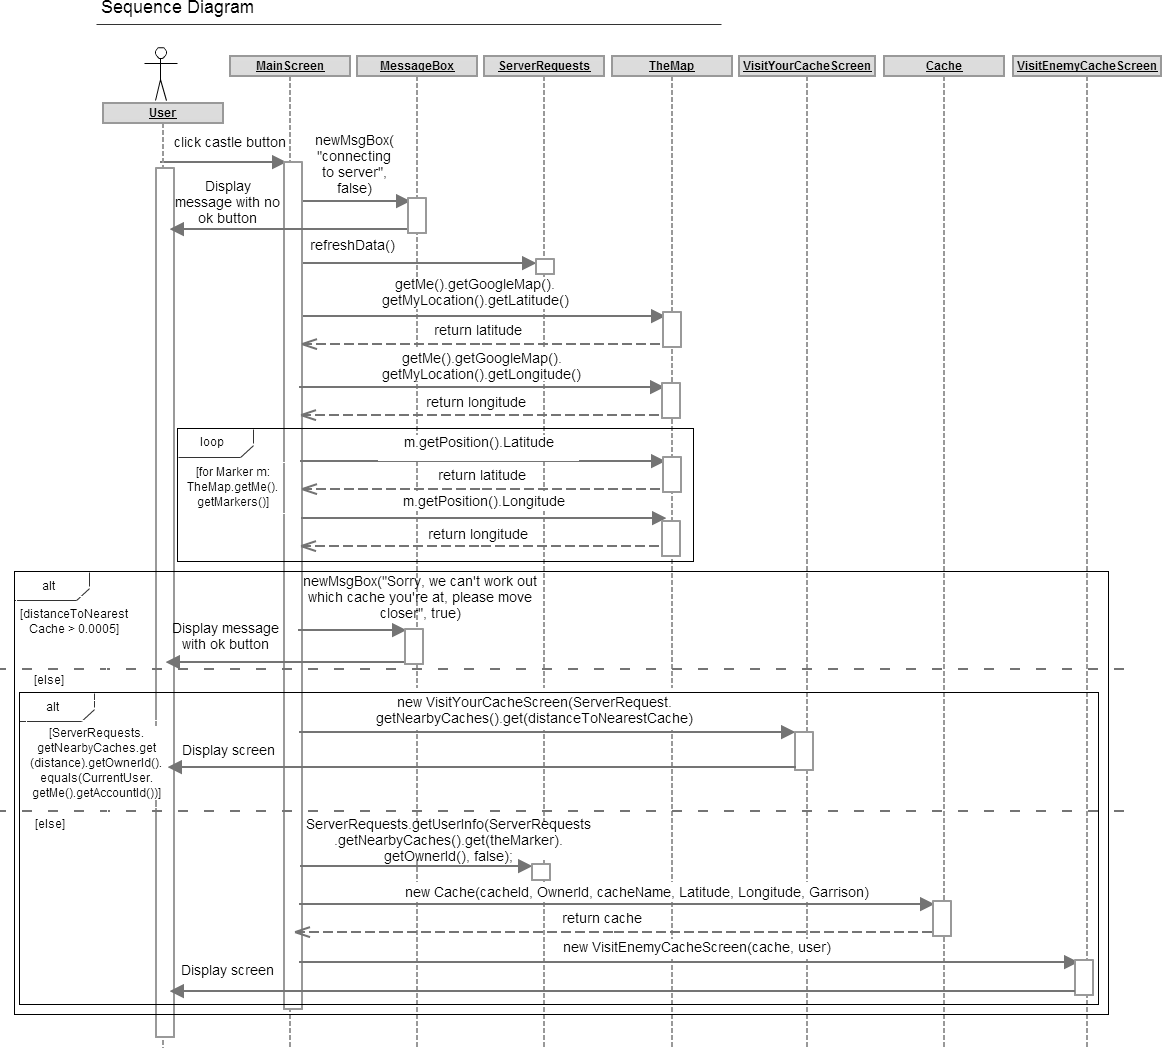
\includegraphics[width=0.9\textwidth]{images/sequence/castleButton}
    \caption{Sequence diagram for the context sensitive castle button.}
    \label{fig:castleButton}
\end{figure}

As previously said the IconUpdater class decides whether the castle button is clickable and also what image is displayed for it. Once created, it runs in the background of the app unless it's told not to. While it hasn't been told to stop running it tries to get the position of the user and the positions of caches. If any cache is close enough then if the main screen is displayed the castle icon is viewed as not greyed out and made clickable. Else if no cache is close enough and the main screen is displayed the icon is viewed as greyed out and changed so when clicked nothing happens. If IconUpdater gets an error doing any of this more than 10 times the user is told that the IconUpdater has crashed through a message box.

\newpage
\begin{figure}
    \centering
    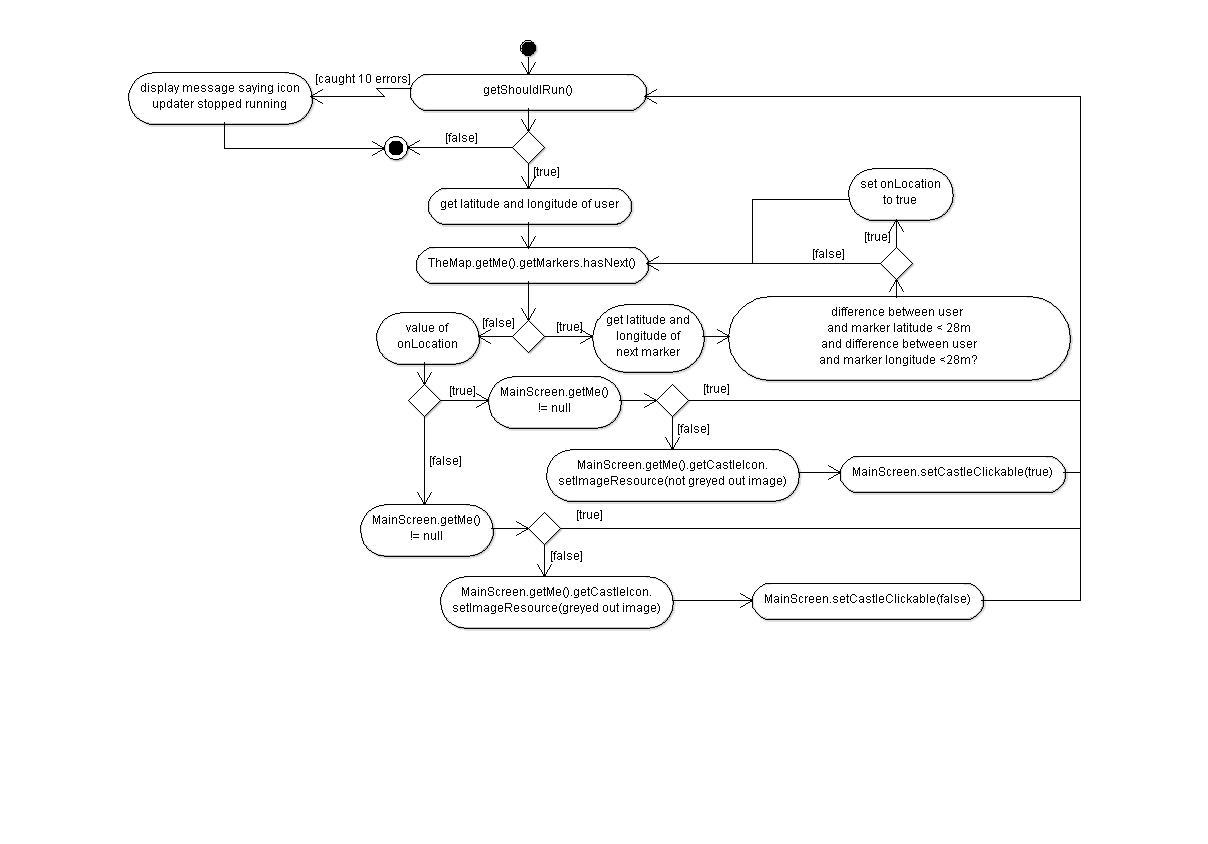
\includegraphics[width=0.9\textwidth]{images/activity/iconUpdator}
    \caption{Activity diagram for the castle button icon updater.}
\end{figure}

The castle button is used to attack and scout caches. When the scout cache button is clicked the app checks it can access the phone's location and Google maps. If it can't it will tell the user the problem else the user is told they are being connected to the server. The user sends a request to the server to scout a cache using the phone's location, the users chosen number of scouts to send and the cache ID. If there is a problem then it is explained to the user. The server is then asked to refresh the data so any scouts that are lost are updated on the app. Again the user is told any problems. When the first request was sent a response was made and the app analyses this to find out which screen to display next. If all the scouts sent were lost the scout failure screen is displayed else the scout success screen is displayed. This satisfies requirement 5.2.9 cache scouting.

\newpage
\begin{figure}
    \centering
    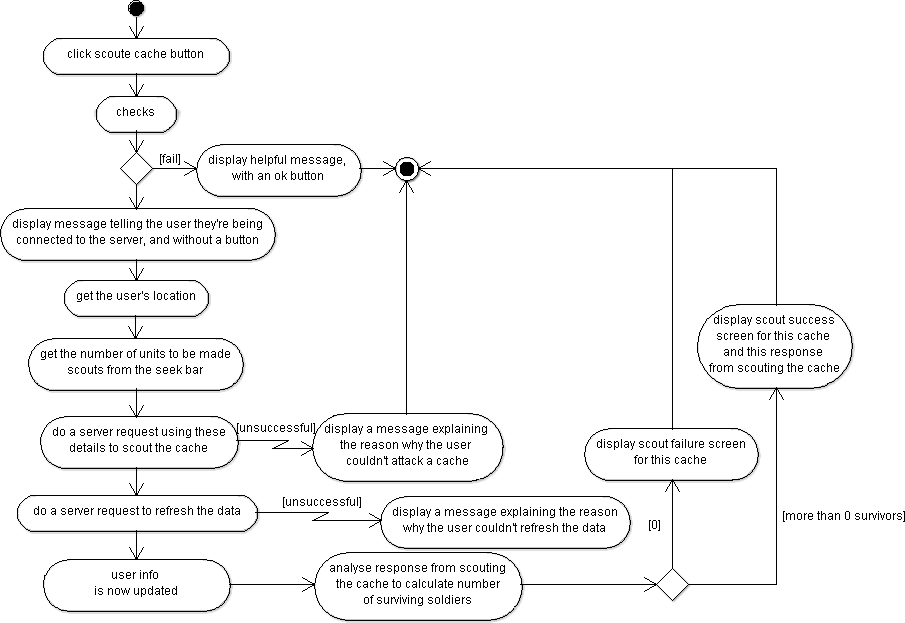
\includegraphics[width=0.9\textwidth]{images/activity/scout-cache}
    \caption{Activity diagram for the cache scouting interface.}
\end{figure}

A user can attack caches by clicking on an attack cache button. The app checks the location can be found and tells the user if their location can't be found. If it can be found the user is told they're being connected to the server. The user's location, number of units they wish to fight with and the ID of the cache are used to make a server request to attack a cache. The server is then requested to be refreshed so all the data can be changed based on the outcome of the attack such as the new cache balance from the remaining defenders or attackers and the owner of the cache. This satisfies requirements 5.2.11 successful attack and 5.2.12 successful defence. If there are any problems with these requests the user is told. If not the user is displayed the post battle screen which processes and displays the response from the first server request, which will satisfy requirement 5.2.13 battle breakdown. This satisfies 5.2.10 cache attacking. Attacking non-player caches is very similar, however the refreshing data might change whether or not the cache is viewed on the map if the user wins the battle, also the owner and cache balance will never change. This satisfies the requirements 5.2.17, 5.2.18, and 5.2.19.

\newpage
\begin{figure}
    \centering
    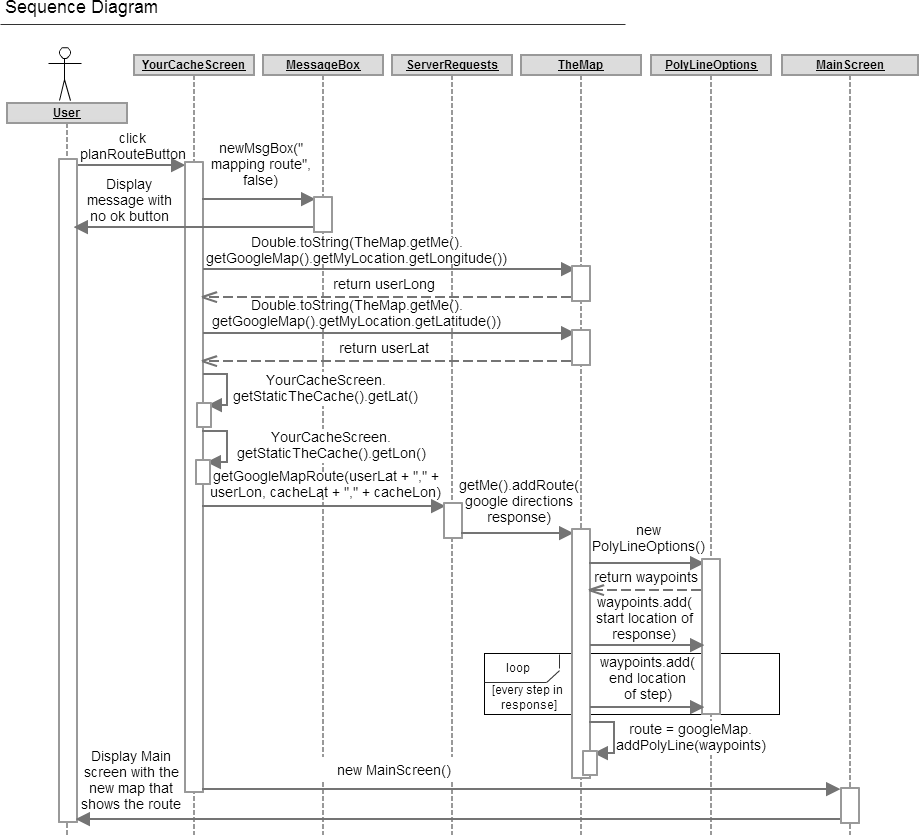
\includegraphics[width=0.9\textwidth]{images/sequence/getRoute}
    \caption{Sequence diagram for the route finding feature.}
    \label{fig:getRoute}
\end{figure}

A user can get to caches using a plan route button. In figure \ref{fig:getRoute} I've used the one on YourCacheScreen as an example but you can similarly plan routes to enemy caches. Firstly when the user clicks the button their location is checked and if it can't be found they are told. If not they are told the route is being mapped. TheMap class is used to find the users location and the class of the screen they're on is used to find the caches location. The locations are used as Strings for the getGoogleMapRoute() method in the ServerRequests class. This calls the addRoute() method in TheMap class with the response received. This method uses a predefined class to create waypoints out of the response and join them up on the map to make a route. Lastly the user is taken to the MainScreen with the route on the map. This satisfies requirement 5.3.4 path finding.

\newpage
\begin{figure}
    \centering
    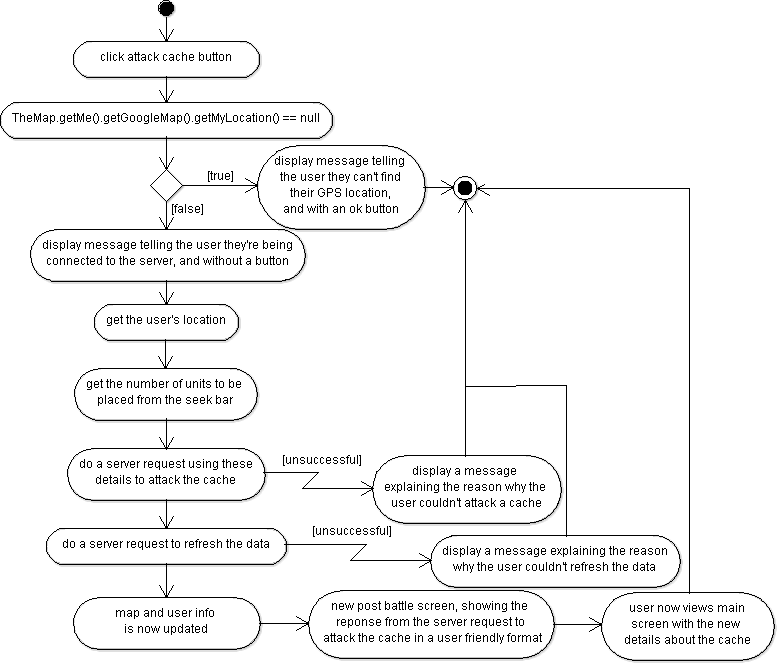
\includegraphics[width=0.9\textwidth]{images/activity/attackCache}
    \caption{Activity diagram for the cache attacking interface.}
\end{figure}

A user can place a cache by clicking the flag button. If their location can't be found they are told else they are told they're being connected to the server. A server request is made using the user's location and number of defenders they wish to make defenders for the cache to be placed. If this is unsuccessful e.g. due to an error or being too close to another cache then the user is told else the server is requested to refresh the data for the new cache to be added. Again if this is unsuccessful the user is notified why, else the user goes to a new main screen with the map now showing the cache. This satisfies requirement 5.3.5 cache placement. Note: when a cache is placed there must be at least 5 units in the seek bar, 4 of which will be lost. This satisfies requirement 5.2.8 cache placement cost.

\newpage
\begin{figure}
    \centering
    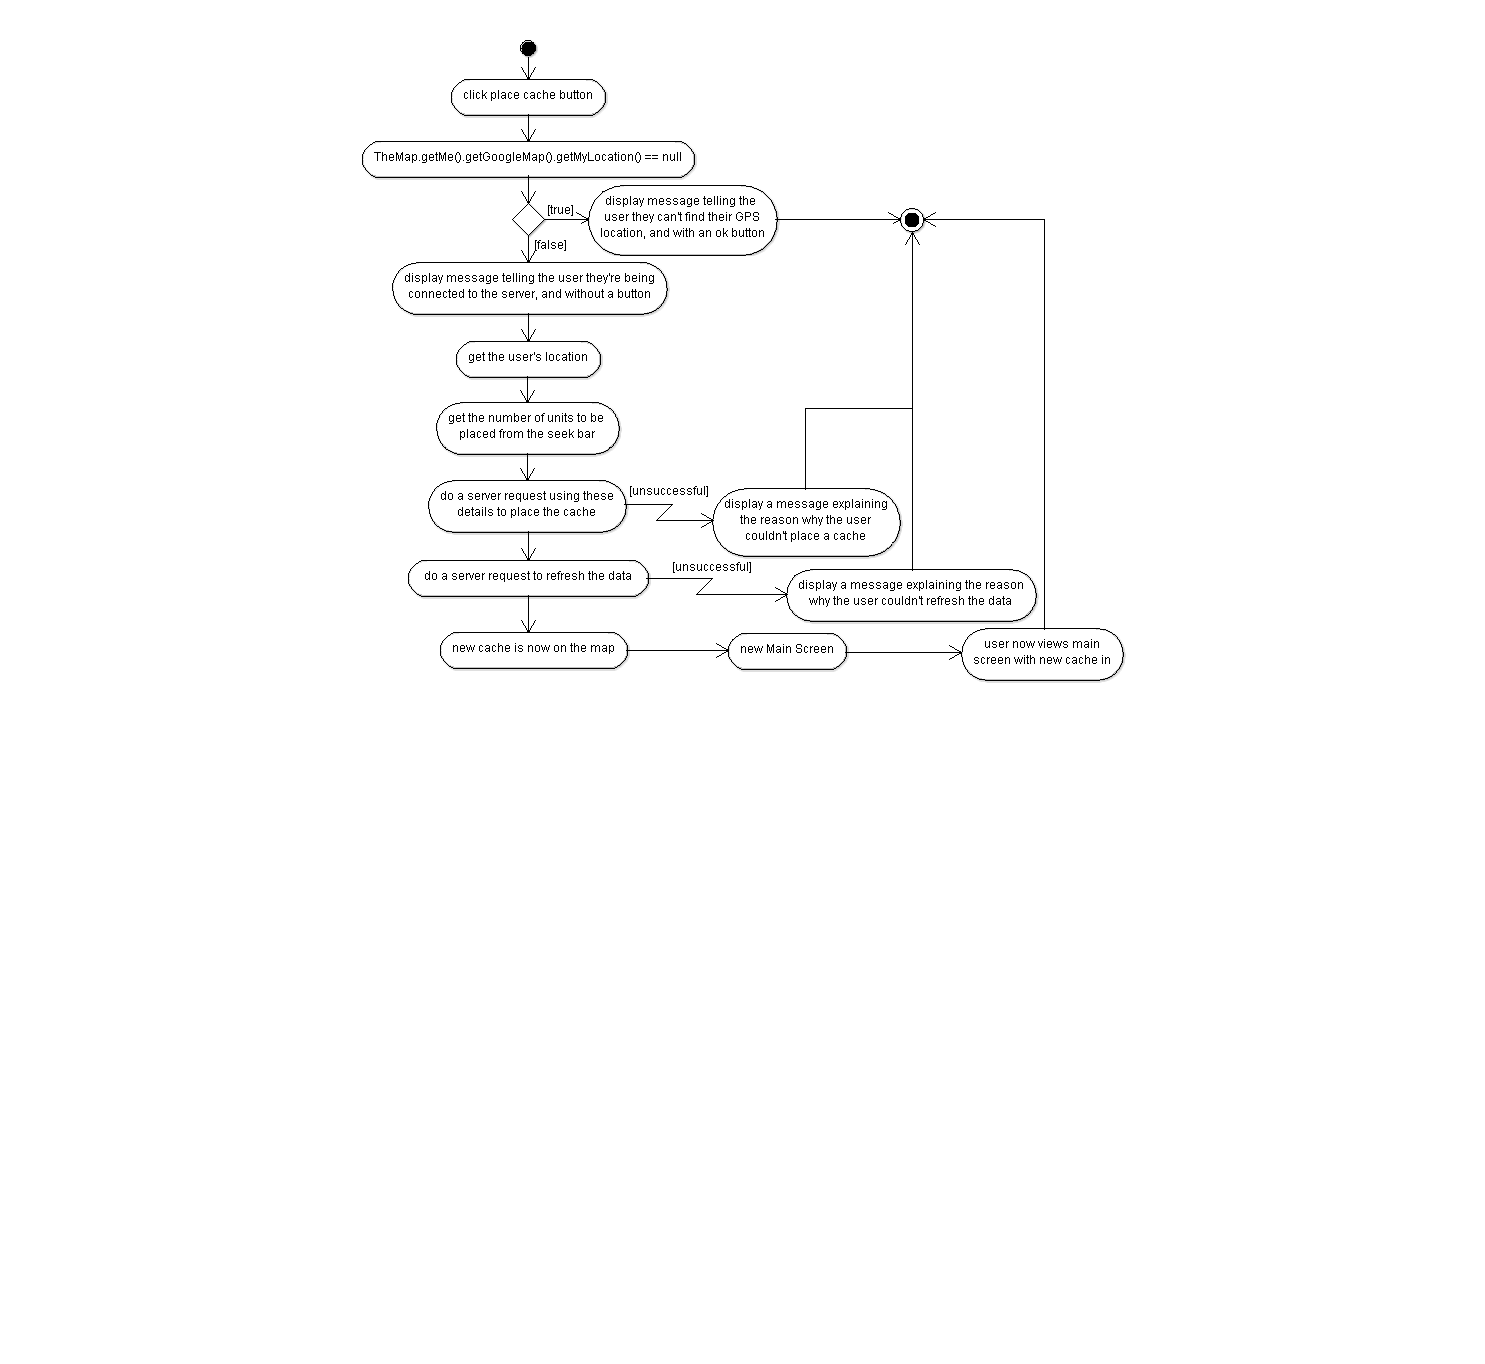
\includegraphics[width=0.9\textwidth]{images/activity/placeCache}
    \caption{Activity diagram of the cache placement interface.}
\end{figure}

On the cache transactions screen the user can withdraw and deposit soldiers from the cache. When the submit button is pressed the users location will be found and if it's null then the user will be displayed an error message, if not they will be told they're being connected to the server. The number of units to be withdrawn or deposited will be found from the seek bar, ServerRequest.cacheTransactions() will be called then ServerRequests.refreshData(), to be able to view the changed balances. If any errors occur in the ServerRequest methods then the user will be explained the error in a message, else they'll be taken back to the main screen. This will satisfy requirement 5.2.5, and 5.2.7. If the user withdraws all the troops then the cache will become unowned satisfying requirement 5.2.6. Unowned caches will have a separate screen from which users can place soldiers in to own that cache, further satisfying requirement 5.2.7.

There is a messaging feature in the app, which can be navigated around from the inbox screen. This screen will be made like most other screens except for the buttons to particular messages, where a few more classes need to be involved before adding these to the grid. Firstly the information about the 7 viewable messages are set using ServerRequests.setMessages(username, when). The when variable is used to tell which 7 messages are used, for example if the user clicks next twice then the 3rd set of 7 messages will be used, then if the user clicks previous the 2nd set of 7 messages will be used. There will be checks in place to stop `when' being invalid for example negative or so large there are no messages in the set. The message information is used to decide what the icons look like and the text displayed. This satisfies requirement 5.4.1 user communication.

\begin{figure}
    \centering
    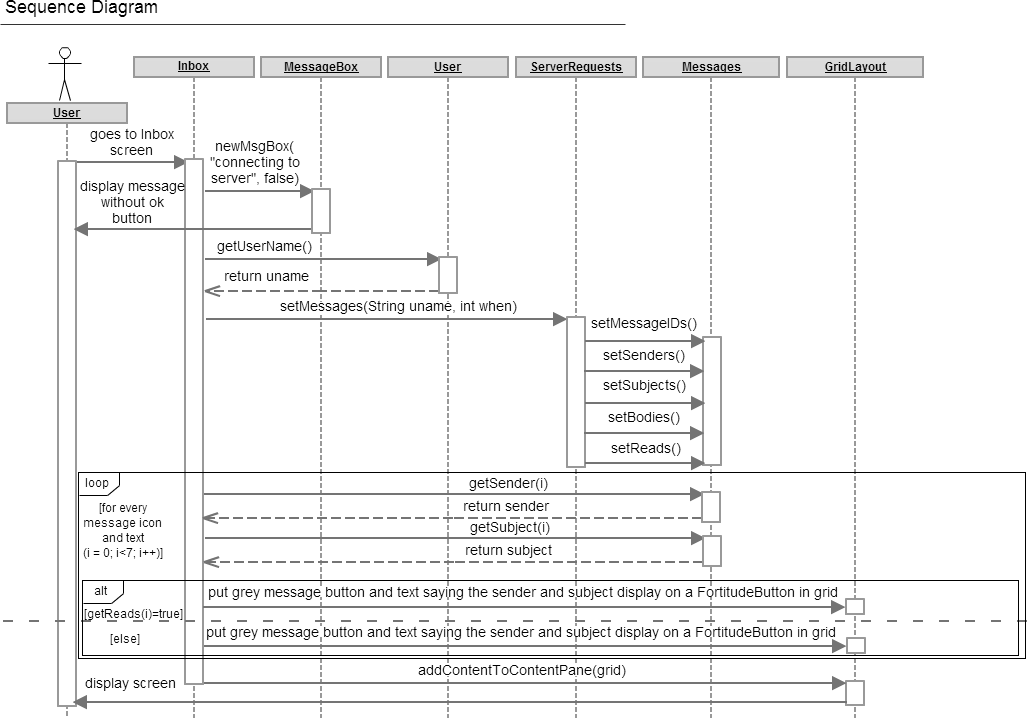
\includegraphics[width=0.9\textwidth]{images/sequence/inbox}
    \caption{Sequence diagram of the messaging feature.}
\end{figure}

When a user clicks an icon to go to a message the variables related to currentMessage are set to those from the corresponding message in the array in the Messages class and if currentMessage.getRead() is false then ServerRequest.setRead(currentMessageID) is called and currentMessage.setRead(true). The values in currentMessage are then used to view the message screen, to automatically put the correct user in the `send to' box when replying and to feed into the server request reportMessage if a user wishes to report the message. This satisfies requirement 5.4.2 communication reporting.

Cache reporting works much like message reporting and is done through the same screen. When reporting a cache, the screen will have a subject and description relating to caches rather than messages, and when submit is pressed reportCache() in ServerRequests will be called with the cache, the user and the text that was entered as parameters. This satisfies requirement 5.2.22 cache reporting.

Users can block other users through the settings menu in messages and through the EnemyProfileScreen account screen. When a user is blocked, User.getBlockedUsers() is called to check if the user is already blocked and if not User.addBlockedUser(String username) is called then the method blockUser(String userBlocker, String userBlocked) is called in ServerRequests. The information is stored in the app and server as it will speed up loading screens to have it in the app while it has to be in the server so when other users messages aren't sent they can be notified. When a user is unblocked, the User class checks they are blocked are removes them from the list of blocked users using User.removeBlockedUser(String username), then the method unBlockUser(String userBlocker, String userBlocked) is called in ServerRequests. A user is blocked and unblocked using the same button in the EnemyProfileScreen so when this screen is made and the button is pressed User.getBlockedUsers().contains(String username) must be called to decide which button is displayed and what action is taken. In the settings menu of messages a list of blocked users are displayed so whenever this screen is initialised the User class is used to find the names and whenever a user is blocked or unblocked the screen must be reloaded. When a user sends a message to a blocked user, the message will still be sent to and stored in the server however the user will be shown a message box saying the message was unable to send.

There is a recent news screen which works much like the inbox screen. When it is initialised setActivity(String username, int when) from the serverRequests class is called to add the information needed from the server. It creates button rows that have different text and icons using this information. It also stores the JSON responses on the app so that when a row is clicked the user can go to the right screen. If the boolean corresponding to the row clicked in isMessage is false then the cache is extracted from the corresponding response using get(``cache'') and this and the response is used to display the post battle screen. If the corresponding value in the isMessage array is true then values for sender, subject and body are extracted and stored as the corresponding current message variables in the Messages class and used to view the message screen. This satisfies requirement 5.3.6 activity recording.

\begin{figure}
    \centering
    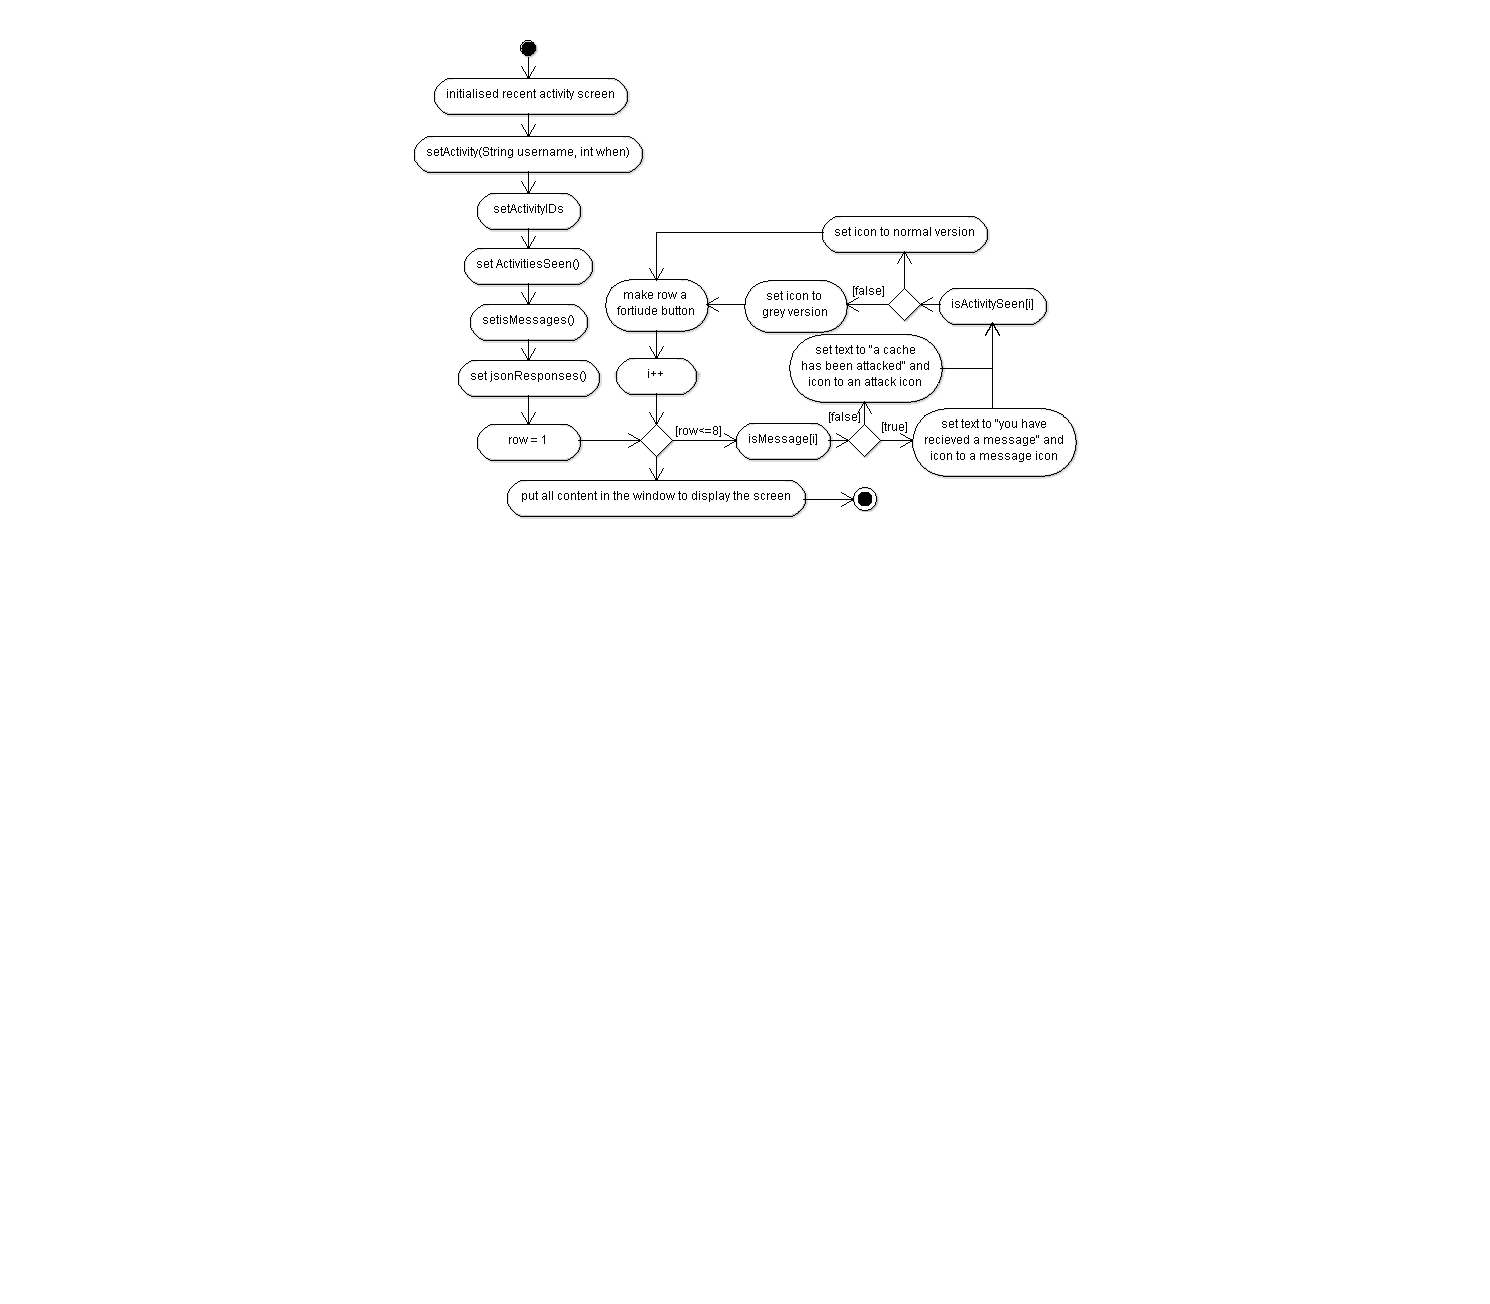
\includegraphics[width=0.9\textwidth]{images/activity/recentActivity}
    \caption{Activity diagram of the recent news list.}
\end{figure}

Special caches will involve the SpecialCacheUpdate class that works much like the IconUpdator class. It is constantly running in the background, getting user's WiFi networks and checking if any have a MAC address of a special cache. If the user can connect to a particular MAC address, then if they are currently on the main screen, the screen will be killed, and the user will be shown the SpecialCacheFoundScreen. From here they can click to claim their prize and if they can still connect to the network with the right MAC address and the reward is still available, they will be displayed a message telling them they were successful, their account will be refreshed so the server knows not to use this special cache in the SpecialCacheUpdate again and the users balance will be updated, which will satisfy requirement 5.2.2 and 5.2.21. If they can no longer connect to the correct network they will be displayed a message saying they were unsuccessful. Either way they will then be taken back to the main screen. This will satisfy requirement 5.2.20, special event placement.

As you can see after user actions that could change data, the data is refreshed which means it will be accurate so a user can see their account balance accurately at any time satisfying requirement 5.2.1 and points can be added or removed from an account balance by other components of the system satisfying requirement 5.2.2. As all user actions involve displaying a message box requirement 5.2.14 cache operation chronology will be satisfied because a message box disables the screen underneath, so the user can't do anything else until the server has finished processing the action.

This section will now take a look at the design of the server. When a request is made in general, the processes in figure \ref{fig:serverGeneral} will occur. The APIManager class will receive a URL from an external source in a form such as /api/scout?uname=Metapyziks\&session=0123456789abcdef. It will use the Request class to find the specific request class needed so in this case it would be the ScoutCacheRequest class. It will then use the method Respond in the specific request class to get a response that is changed into JSON form and sent back to the external source. However if a specific request class can't be found then the ErrorResponse class is used. The server is not going to involve threading so each task will be carried out one at a time to satisfy requirement 5.2.14.

\begin{wrapfigure}{l}{0.6\textwidth}
    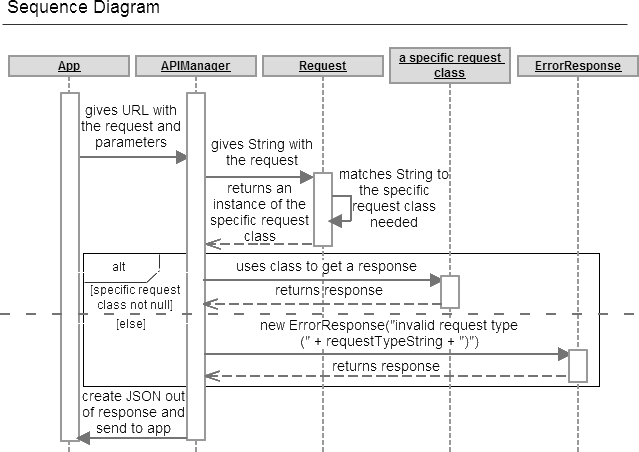
\includegraphics[width=0.6\textwidth]{images/sequence/Servergeneral}
    \caption{Sequence diagram of the general server API system.}
    \label{fig:serverGeneral}
\end{wrapfigure}
The following sequence diagram shows how the specific request class RegisterRequests is used to get a response. Firstly the method attemptRegister() is called in the account class. This method will perform the checks needed to satisfy requirement 5.1.1: Account Registration. If any of these checks are failed then a related instance of ErrorResponse will be returned. If the checks are passed then a new account will be made with the username, email and password hash supplied, the rank as unverified, the registration date set to the current time, the activities list set to a new list of Response, the blocked list as a new list of String and the dictionary of non-player caches found created. (The rank can be changed to Administrator which satisfies requirement 5.1.3: Administrator Accounts) This account is placed in the database and used as a parameter in EmailValidationCode.create() along with the Enum EmailValidationType set to Activate. The code created is used to send an email to the user to activate their account, which will satisfy requirement 5.1.2:Account Activation. If it has got to this point in the method then null is returned so the Response is made using the Response method which gives a successful response rather than an error.

\begin{figure}
    \centering
    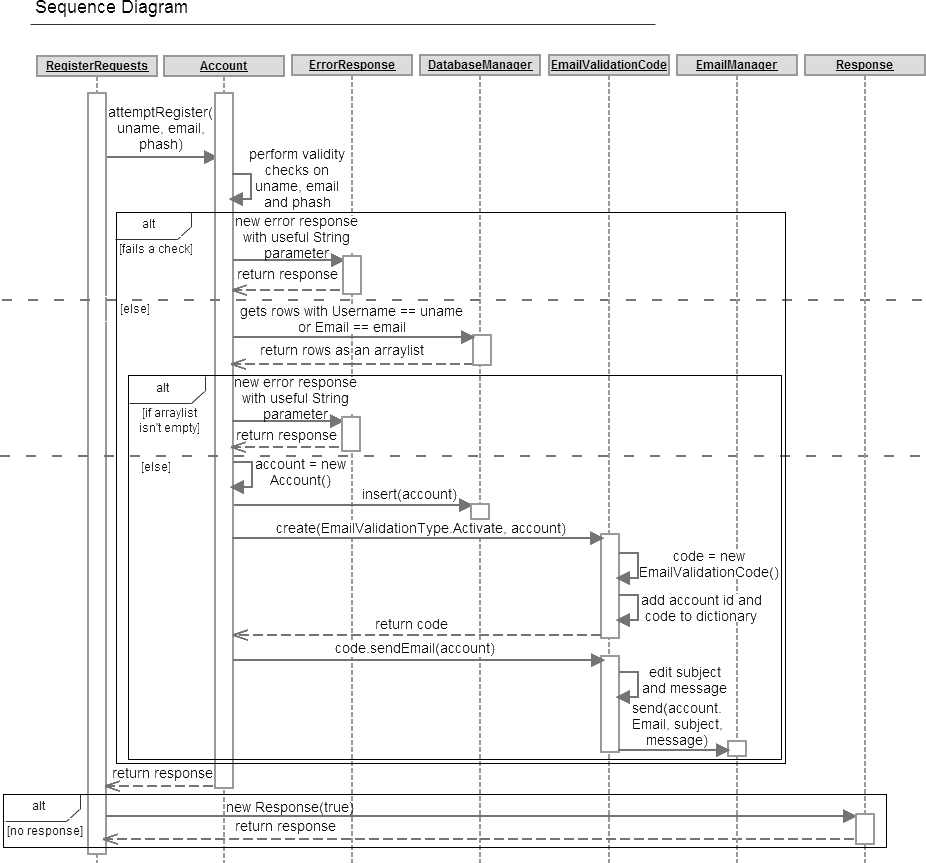
\includegraphics[width=0.9\textwidth]{images/sequence/registerUser}
    \caption{Sequence diagram of the user registration process.}
\end{figure}

\begin{wrapfigure}{r}{0.45\textwidth}
    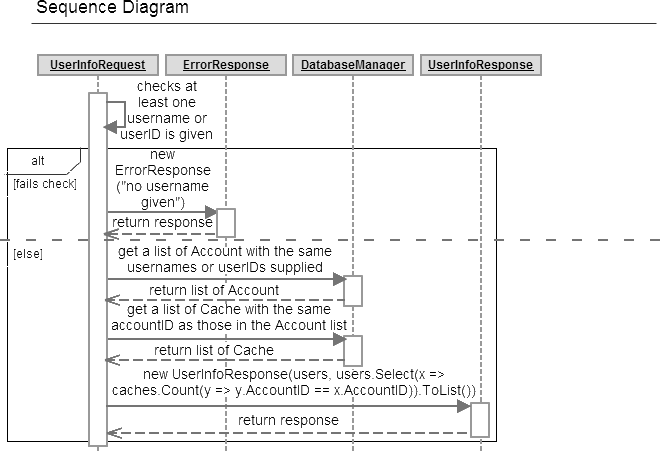
\includegraphics[width=0.45\textwidth]{images/sequence/userinfo}
    \caption{Sequence diagram of the user information request.}
    \label{fig:userInfo}
\end{wrapfigure}

When resending an activation email it is the SendActivationRequest class that performs checks to satisfy requirement 5.4.1: User Communication. The account with the email address provided is selected from the database and used to resend an activation email in the same way as account registration. If an ErrorResponse hasn't already been returned then a Response will be like with account registration.

When sending a password reset email, PasswordResetRequest let's EmailValidationCode perform the checks to satisfy requirement 5.1.8:Password Reset in the method AttemptCreate(). If it passes these checks an EmailValidationCode will be created and used to send an email to the user and a Response will be returned, else if the checks aren't passed an ErrorResponse will be returned.

Figure \ref{fig:userInfo} shows how UserInfoRequest works, as you can see the checks are performed in the specific request class. If passed then the accounts and caches of the users wanted are found. The response is found using this list of Account and a list of Int corresponding to the number of caches the user has. UserInfoResponse uses these parameters to make a response in the form:

\begin{verbatim}
{"users":[{"accounted":0,"uname":"metapyziks","regdate":1347374370,
"rank":Unverified,"caches":0},{"accounted":1,"uname":"TestName",
"regdate":1347381045,"rank":Verified,"caches":23}],"success":true}
\end{verbatim}

\begin{wrapfigure}{l}{0.53\textwidth}
    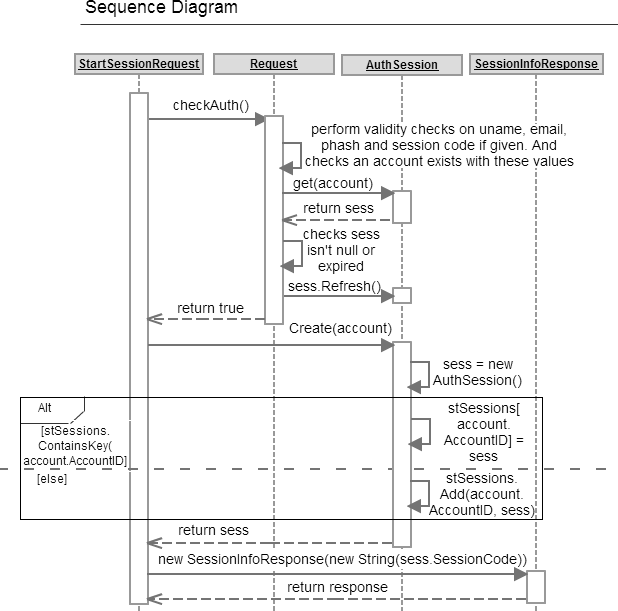
\includegraphics[width=0.53\textwidth]{images/sequence/createSession}
    \caption{Sequence diagram of the session creation process.}
\end{wrapfigure}

The server creates a new session using StartSessionRequest. This performs all the necessary checks on the username, email, password hash supplied with the Request class, which will also get the account corresponding to the user supplied and check the account along with the SessionInfoResponse corresponding to the account. It checks expiration using the method IsExpired() in AuthSession. If any of the checks are failed a related ErrorResponse is initiated and fail is returned to StartSessionRequest which will not go on to do AuthSession.Create(account). If the checks are passed the instance of AuthSession is refreshed which will set the refresh time to the current time so it can be used in the IsExpired() method. True is returned to StartSessionRequest, a new instance of AuthSession is made with an AccountID, SessionCode, LastRefresh set to now and a Rank set to the rank of the account. The AuthSession is added to a dictionary of AuthSession as an update or new entry with a new AccountID. The AuthSession is returned to StartSessionRequest which is used to create a new SessionInfoResponse with a code and success value. This satisfies requirement 5.1.5: User authentication.

The UserStatsRequest class works by checking in the same way as StartSessionRequest using CheckAuth(). If the checks are passed an instance of Player is created using Player.GetPlayer(account), which selects the player in the database with the correct AccountID using Select() in DatabaseManager. If this player doesn't exist yet then a new Player is created with a balance of 0 and AccountID then inserted into the database using Insert() in DatabaseManager (see scouting figure). The caches the user owns are found using Select() with the caches AccountID as the as the account's AccountID. caches.Sum() is used to find the number of points stored in all the caches owned by the account holder and this along with the player Balance and cache Count is used to create a new UserStatsResponse. This satisfies requirement 5.2.1: Account balance.

To list a users' caches, UserCachesRequest is used, which uses CheckAuth() to find errors. If there aren't any errors then a list of Cache is found with the same AccountID as the Account of the specified user using DatabaseManager. The response including the caches' cacheid, ownerid, name, latitude, longitude and garrison is found by new CacheInfoResponse(caches).

To find a list of nearby caches, NearbyCachesRequest is used. This firstly find errors with CheckAuth() then if none are found it will check the latitude, longitude and radius can be parsed as a double and if not make a new related ErrorResponse. Else that latitude, longitude and radius are used for Cache.FindNearby() which uses DatabaseManager.Select() to find a list of Cache in the radius. The balance of the caches not owned by the user are set to -1 so the user can't know about enemy garrisons, satisfying requirement 5.2.4: Cache balance. The balance of non-player caches is set to -2 to make them distinct from other caches, and they will only be put in the response if the user hasn't defeated the cache in a certain amount of time, satisfying requirement 5.2.19: Scouting Non-Player Caches. Again CacheInfoResponse is used if there wasn't an ErrorResponse needed. This satisfies requirement 5.3.2:Nearby caches.

When a cache is scouted, the ScoutCacheRequest class is used. Checks's are made using checkAuth(), by trying to parse the Strings representing numbers (e.g. units and latitude) into Doubles, and by seeing if the numbers are in the right bounds e.g. positive or smaller than the user's balance. Tools.getDistance() uses trigonometry to find the distance between the user and closest cache. Tools.CoinToss used to calculate the survivors, it creates a random number and if this number is less than 0.8, true is outputted. This is done for every soldier in the scouting army and the number of trues outputted equals the number of survivors. The players balance is set to balance – units + survivors and this is updated in the database. A new ScoutCacheResponse is made with the CacheID, Scouts set to units, Survivors and Garrison set to cache.Balance. The response will include cacheid, ownerid, cache name, latitude, longitude, garrison and success. The response will be put in Activity, the list of responses in the corresponding Account class and updated in the database. This satisfies requirement 5.2.9: Cache scouting.

\begin{figure}
    \centering
    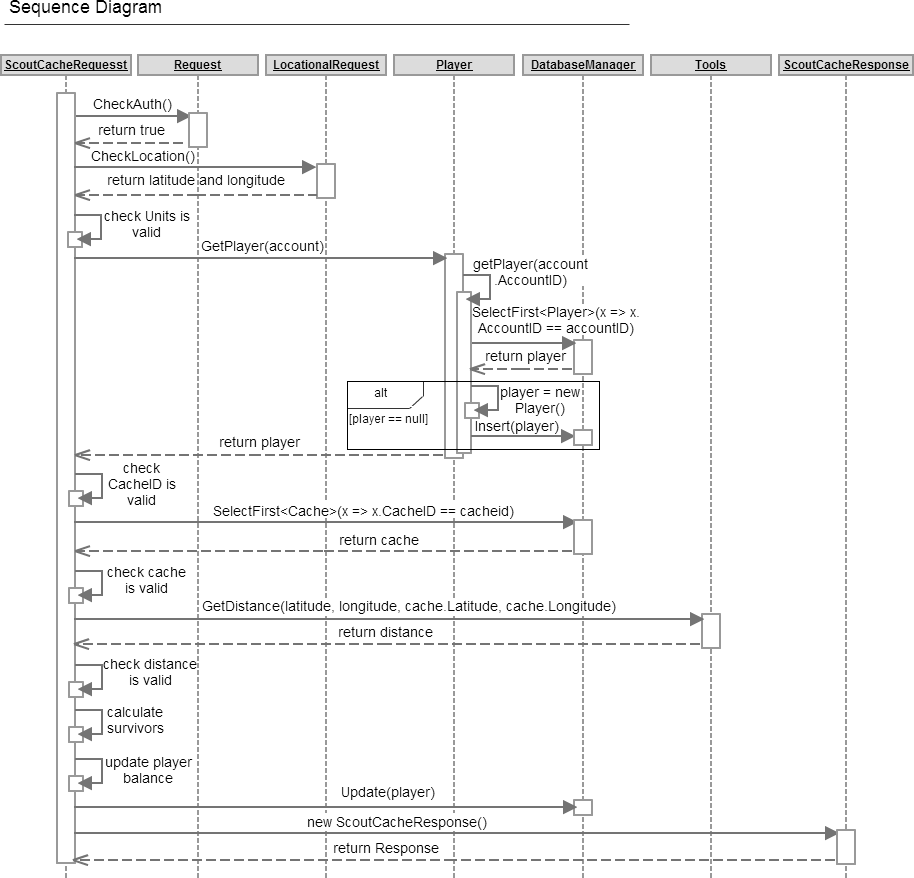
\includegraphics[width=0.9\textwidth]{images/sequence/scoutCache}
    \caption{Sequence diagram of the cache scouting process.}
\end{figure}

The PlaceCacheRequest class performs checks much like the ScoutRequest class, it does CheckAuth(), CheckLocation(), checks units are a Double, larger than the CachePlacementCost and smaller than the player's balance. CheckLocation() see's if the location hash supplied is the same as the location given which will satisfy requirement 5.2.24 anti-cheating measures. It also uses Cache.FindNearby() which uses as supplied minimum distance, latitude and longitude to find the caches within that distance, and PlaceCacheRequest uses this information to see if the user is far enough away from other cache to place a cache. If all of the checks are passed then a new Cache is made with an AccountID, Balance which is 4 less than units, Latitude, Longitude, Name which is randomly selected, CacheID which isn't supplied by PlaceCacheRequest and Nonplayer set to false. The Cache has an associated AccountID to satisfy requirement 5.2.3: Cache ownership, and a Balance to satisfy requirement 5.2.4: Cache balance, which is less than units to satisfy requirement 5.2.8: Cache placement cost. The players balance is updated and saved in the database, and the cache and activity is inserted into the database. A new CacheInfoResponse is made which includes cacheid, ownerid, name, latitude, longitude, garrison and success. This satisfies requirement 5.3.5: Cache placement.

\begin{figure}
    \centering
    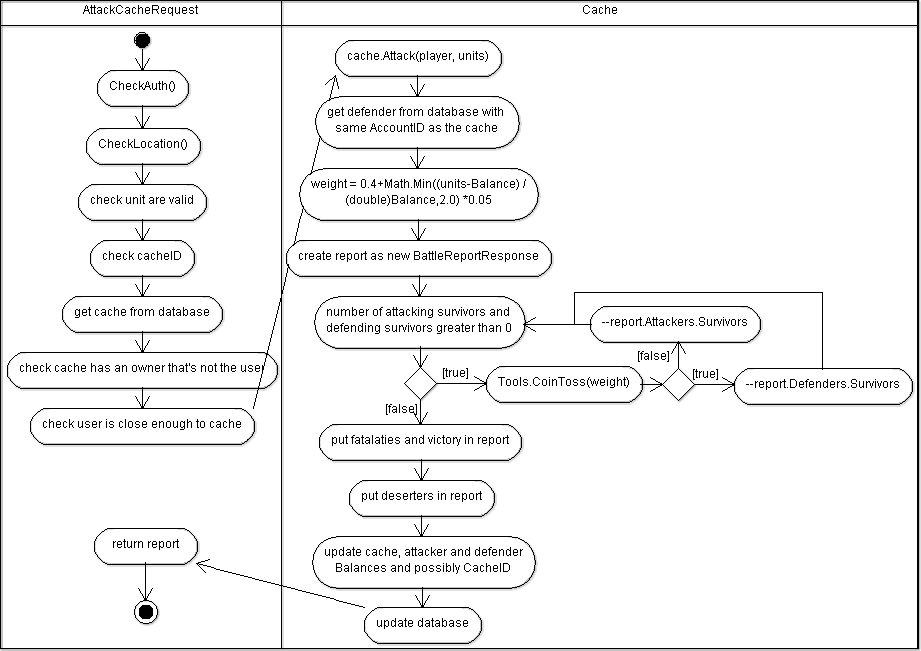
\includegraphics[width=0.63\textwidth]{images/activity/server_attackCache}
    \caption{Sequence diagram of the cache attacking process.}
\end{figure}

As you can see the checks for attacking caches are done in the AttackCacheRequest class, and the response is created in the Cache class. The sum used for weight is based off an estimate of figures in pre-Saxon Britain. The BattleReportResponse is initially set with the cache, AttackerID, DefenderID, Attackers made from a new BattleReportResponse.UnitReport with Initial and Survivors set to units, and Defenders made from a new BattleReportResponse.UnitReport with Initial and Survivors set to cache Balance. The fatalaties are put in the report with report.Attackers.Fatalities = report.Attackers.Initial – report.Attackers.Survivors and a similar method for Defenders. Report.IsVictory is true if there are attacking survivors, in this case report.Attackers.Deserters = 0 while the defending deserters are a small random proportion of the defending fatalities, the cache Balance becomes the surviving attackers plus the defending deserters and the caches AccountID becomes the attackers AccountID. However if IsVictory is false, there are 0 defending deserters, a small proportion of the attacking fatalities are deserters, the cache balance is the surviving defenders and the attacking deserters are added to the defenders balance. The response is added to Activity in the affected instances of Account and updated in the database. This satisfies requirement 5.2.10: Cache attacking, 5.2.11: Successful attack, 5.2.12: Successful defence and 5.2.13: Battle breakdown. Attacking non-player caches is very similar, the same request is used, the only difference is that the user's Account NonPlayerDictionary will be updated with the cacheID and time, the `point reward' will be shown as the deserters, which there will be more of to make up for not getting the cache, and the cache balance won't change in the database. This satisfies requirement 5.2.18: Attacking Non-Player Caches.

When a message is sent the MessageRequest class is used, it checks the message body and subject aren't empty. It will create a MessageResponse and put it in Activity of the sender's and receiver's Account and updated on the database. It will check the receiver's Account to see if the sender is blocked and return an ErrorResponse if the sender is blocked else a Response is returned. This satisfies requirement 5.4.1: User Communication.The receiver will always get the message as it is when the activities are requested that the server will make sure that messages aren't received from blocked users. This is so that when a user is unblocked the messages will be received and in the correct order in relation to other activities. There will obviously be a request to block users too which will check the username or id supplied has an associated account that isn't the account of the user before adding the id to the Block list in the user's account. The possible responses are the ErrorResponse or Response. The request to unblock a user is the oppositeto blocking users.

Messages and caches will be able to be reported through the MessageReportRequest and CacheReportRequest classes. They will use the reporterid or username, message or cache id, and a description. They will check the cache or message hasn't previously been reported, and if it's a CacheReportRequest then that it's not the reporter's cache and it's not a non-player cache. The message id is searched for in the reporter's activity to find the message details, or the cache details are found using the cacheid. This information is put into a related Response and added as an AdminResponse in the database so administrators can see it on the website. The cache or message will be marked as reported and saved in the database and a Response will be returned. This satisfies requirement 5.2.22: Cache Reporting and 5.4.2: Communication Reporting.

In many requests the DatabaseManager and Account classes are used in conjunction with the specific request class, with this requirement 5.2.2: Account transactions and 5.3.6: Activity Recording can be fulfilled. There will also be a Request class for getting activities that uses the users Account ID or username, how many activities they wish to see, which set of they want, and what type. It performs checks (including removing messages from blocked user's from the response) and uses modular arithmetic to select the correct set of activities of the right type and return them in ActivityResponse. Requirement 5.2.5: Cache transactions is fulfilled in the same way as 5.2.2 but with Cache class, the request used to withdraw and deposit soldiers will also set the cache owner to null and update it in the database if all the soldiers are withdrawn. This will satisfy requirement 5.2.6: Cache Withdrawal.

\begin{wrapfigure}{r}{0.53\textwidth}
    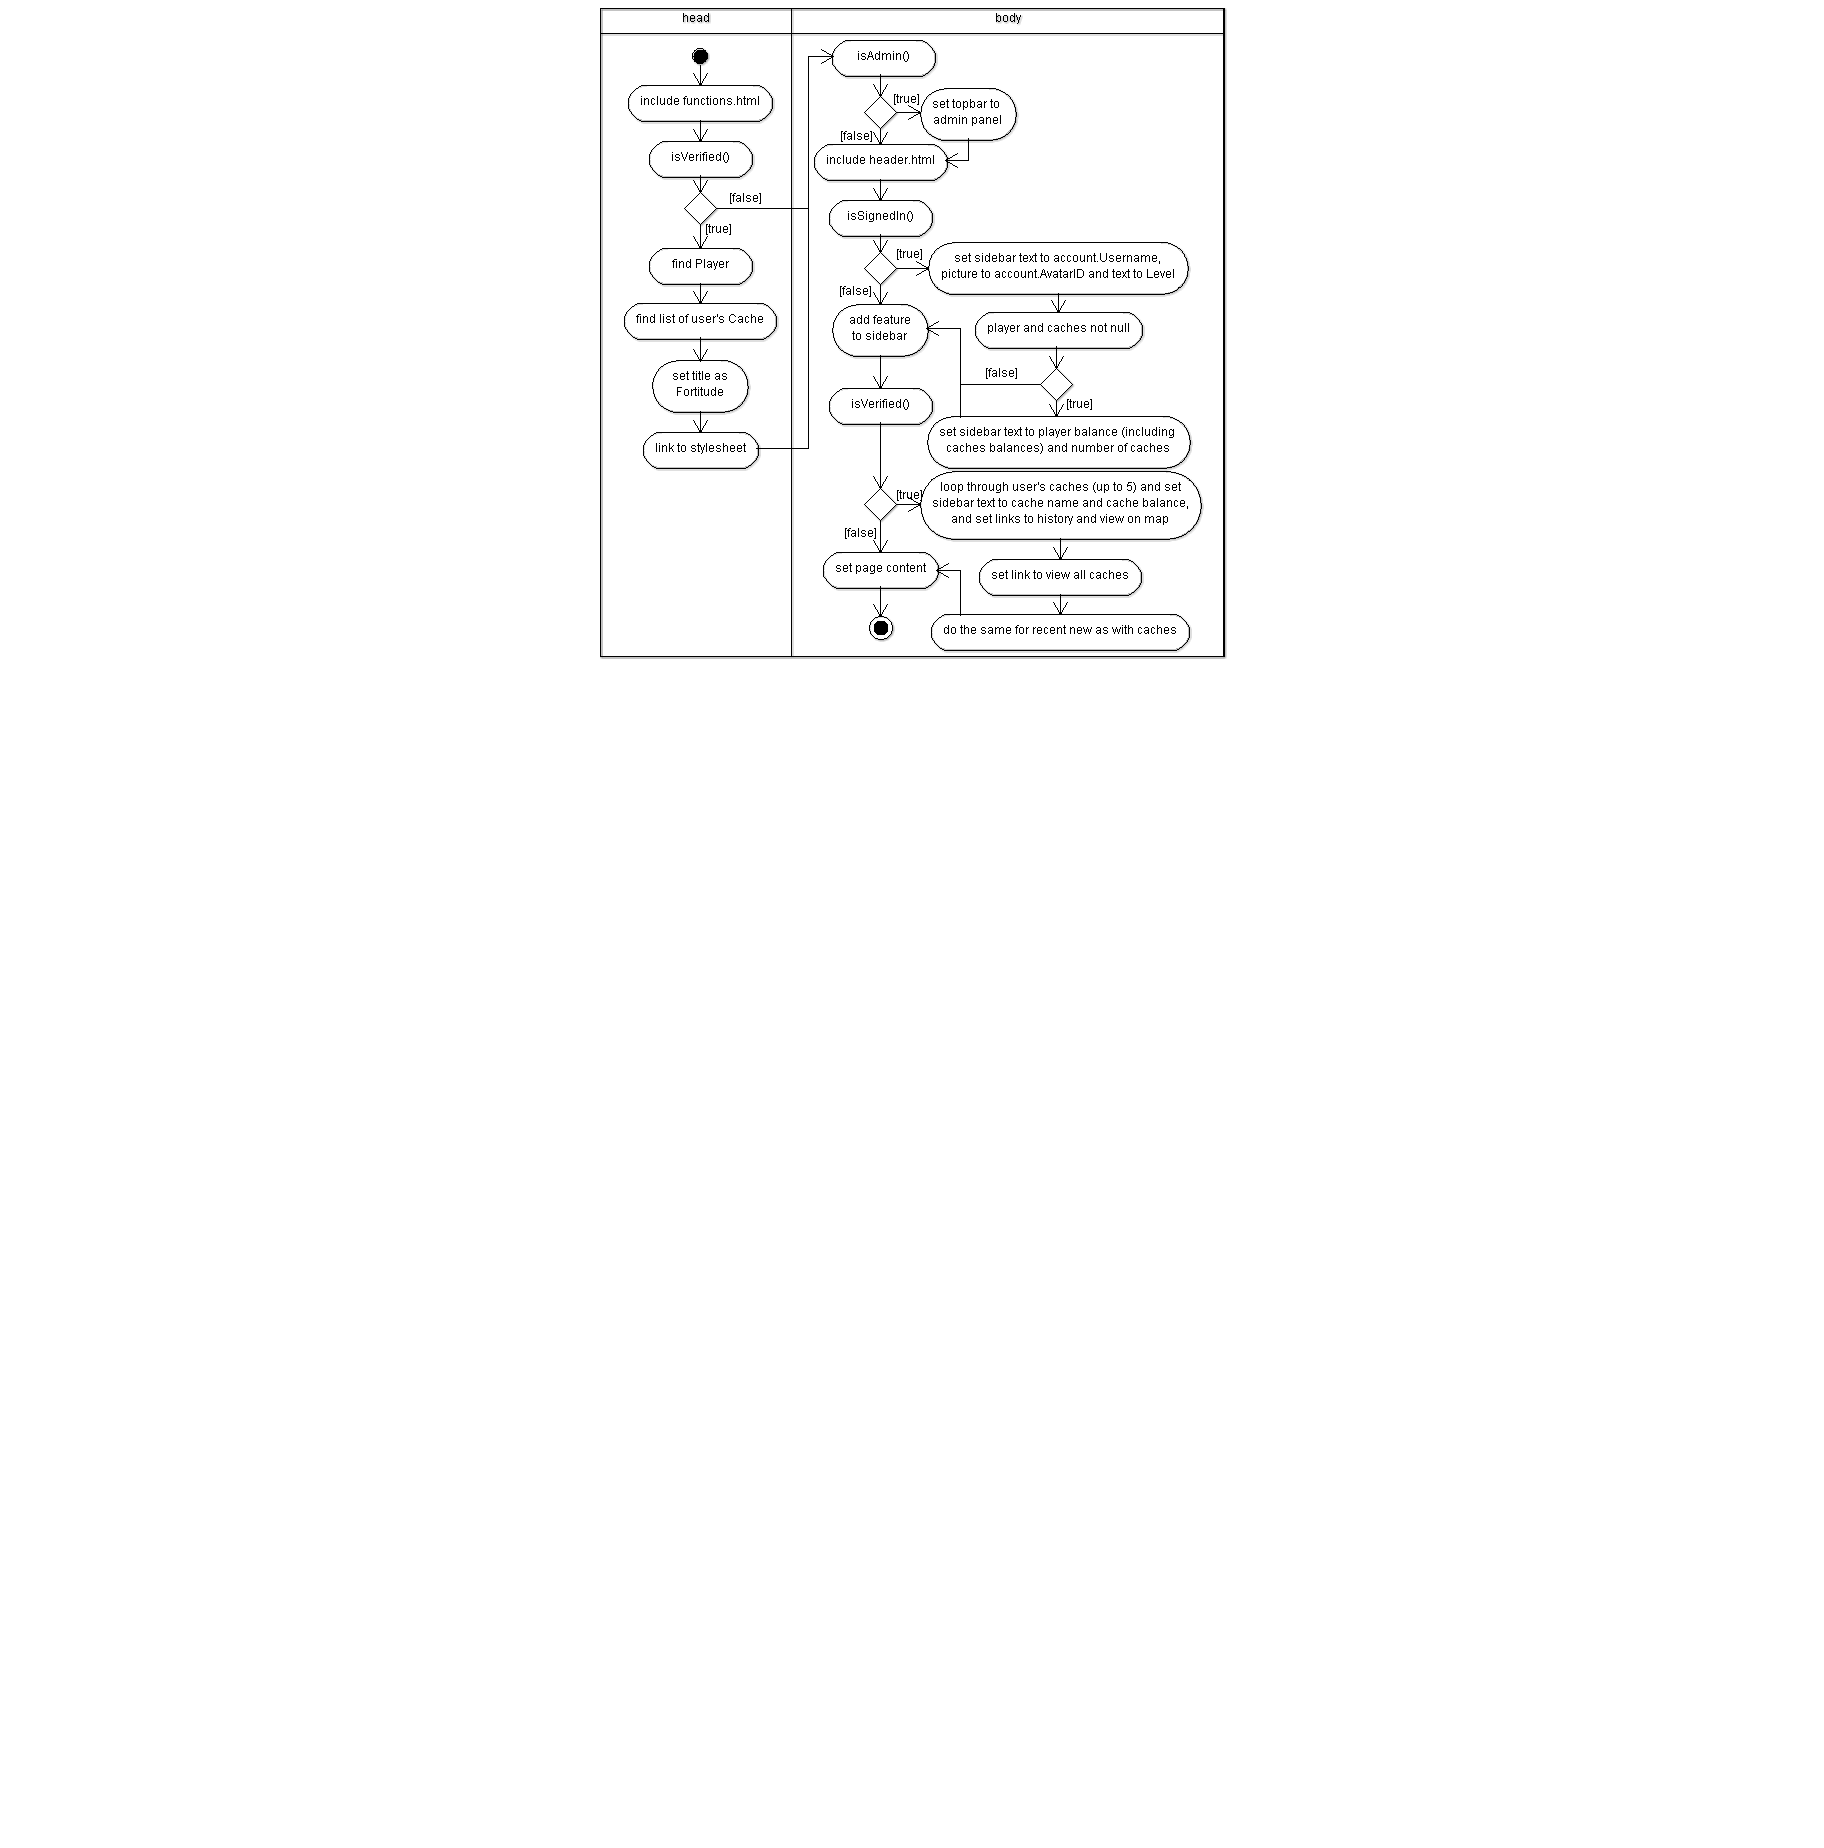
\includegraphics[width=0.53\textwidth]{images/activity/IndexHTML}
    \caption{Activity diagram of the index page construction.}
\end{wrapfigure}

The design of the website will now be discussed. Although not all pages are mentioned, the pages not mentioned will feature forms, checks and updates much like the pages which are examined in detail. This will satisfy requirement 5.4.3: Website.

The index page is made as followed, firstly the header is used to find information needed. It includes function.html which provides a list of methods used for checking such as isAdmin() and pluralify(). If the Account of the user is verified then the Player and Cache classes are used to find the player and their caches. If the account has the rank admin or higher the admin panel is displayed along with the header everyone can see. If the session isn't null (ie isSignedIn()) then the side bar is personalized, and if the player and caches aren't null it is personalized further with the number of caches and the players balance. If the account is verified and there is a session then caches and news plus links to further information, caches and news are displayed in the sidebar. This sidebar will satisfy requirement 5.4.5: Viewing Owned Caches and 5.3.6: Activity Recording. The links to caches will display pages that satisfy requirement 5.4.6: Viewing Cache Details.

\begin{landscape}
\begin{figure}
    \centering
    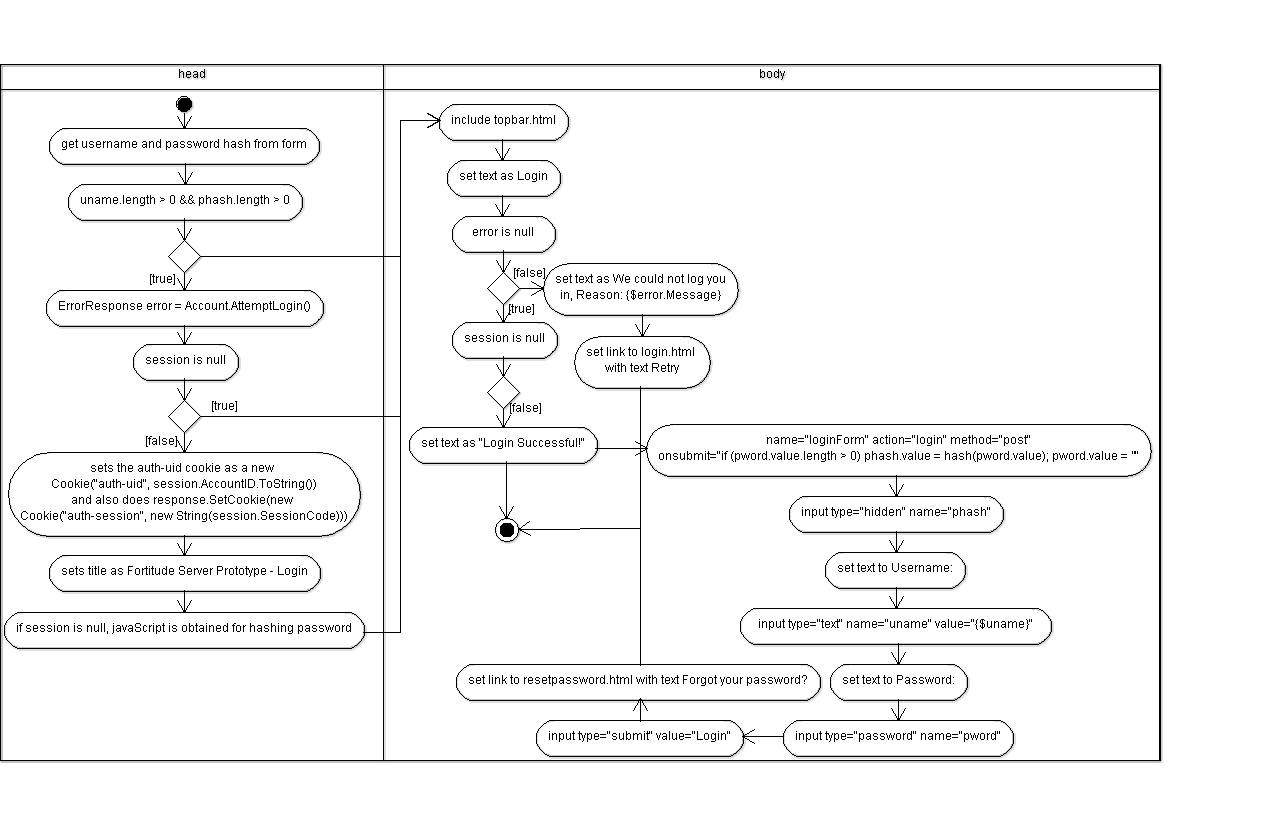
\includegraphics[width=1.1\textheight]{images/activity/loginWeb2}
    \caption{Activity diagram of the login page construction.}
\end{figure}
\end{landscape}

When a user logins in with the website login.html is used. It's head uses the username and password in the form to attempt to login, which will output a session. If the session outputted by Account is null a new session is made using cookies. The title is set and if necessary JavaScript is loaded for hashing passwords. The top bar is added, the subtitle set to Login. If there's an error then it is explained and a link is displayed to try again. If the session is null a form is produced for the user to enter their username and password, which will be hashed. A link is also provided in the case that the user forgets their password. If the session is not null then text will be displaying saying successfully logged in. This will satisfy requirement 5.4.4: Website Authentication.

When a user clicks a link in an email to activate their account activate.html is used. In the head, there will be AttemptActivate(get["email"], get["code"] ) and the title will be set to Fortitude Server – Account Activation. In the body, a sub-title will be set as Account Activation. If AttemptActivate outputted an error that wasn't null then the user is explained the error, if not the user is told their account has been activated and they can now log on. A link will be provided to the Home page at the bottom of the body. This will satisfy requirement 5.1.2: Account Activation.

Admins can place a cache with placecache.html. In the head this checks whether this session is null and the rank of the session. If the session is null or the rank less than administrator the user is redirected to the error page. Else the account corresponding the username submitted is found and checked, if anything fails an error message is set. Else a new Cache is created and updated in the database. The title is set to Place Cache and a form is created to input username, latitude, longitude and units. If success is true then text is displayed saying where the cache was placed else if there was an error, the message is displayed. This satisfies requirement 5.2.16: Administrator Placed Caches. placenon-playercache.html is very similar except the form will only include inputs for position and units. The cache created and added to the Server will have the AccountID as the administrator's AccountID. placespecialEvent.html is also similar, in the head it will be checked if the supplied MAC-address is valid and the number of user claiming the reward and the reward is greater than 0.

These will be in the form in the body. Then the special event cache will be placed in the database. This satisfies requirement 5.2.20: Special Event Placement.

Administrators can delete caches using deletecache.html, this will redirect the user to the error page if their session is null or rank not high enough. It will use the cacheid in the form to get the cache from the database, which will be checked to exist then removed from the database. If it doesn't exist then the error String will reflect this. Text is set to Delete Cache and a form is created for the user to submit Cache ID. If success is true the user is told which cache was successfully removed by name and cacheid. However if there was an error text is set to this error. This satisfies requirement 5.2.23: Administrator Cache Deletion. deleteAccount.html works in a very similar way, it is an admin only page and when the account is removed from the database, all the caches with the accountID are found and removed from the database too. This satisfies requirement 5.1.7: Administrator Account Removal. Users can also delete accounts through the website then the email they will receive from an administrator. Once the link in the email is clicked on the users' caches as well as account will be removed from the database.

\begin{figure}
    \centering
    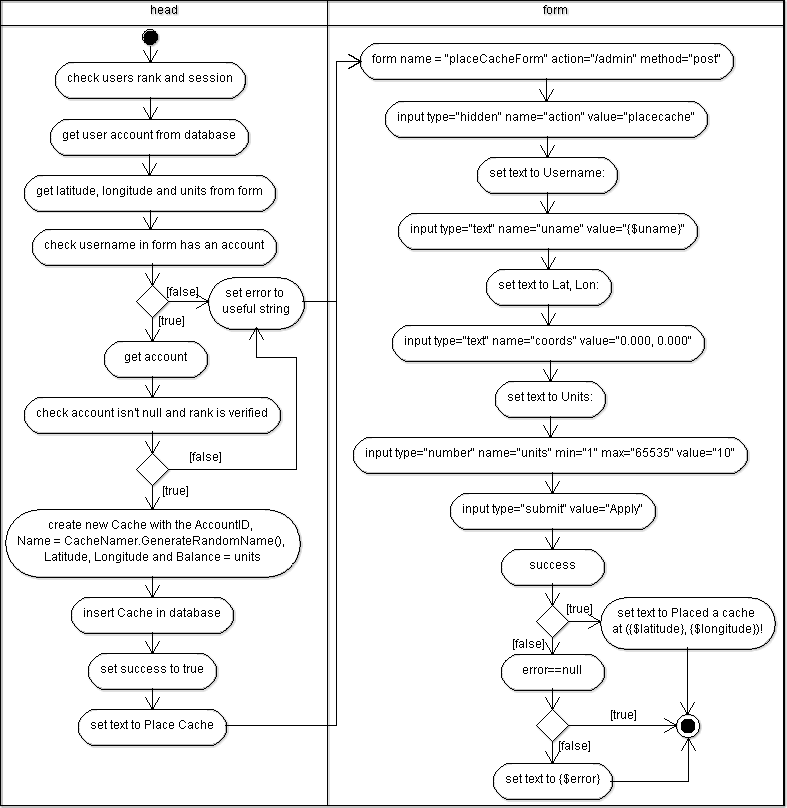
\includegraphics[width=0.9\textwidth]{images/activity/admin-placecache}
    \caption{Activity diagram of the administrator cache placement process.}
\end{figure}
